\documentclass[a4paper]{article}
\usepackage[italian]{babel}
\usepackage{booktabs}
\usepackage{siunitx}%Questo serve a caricare il pacchetto delle unità di misura del sistema internazionale%
\usepackage[utf8]{inputenc}
\usepackage{graphicx} 
\usepackage{url}
\usepackage{amsmath}
\usepackage{amssymb}
\usepackage{listings}
\usepackage{multirow}

\usepackage{keyval}
\usepackage{xcolor}
\usepackage{caption}
\usepackage{subcaption}
\usepackage{subfig}
\usepackage{tikz}
\usepackage{circuitikz}
\usepackage{authblk}
%\usepackage{hyperref}
\lstset{language=C}
\lstset{basicstyle=\small\ttfamily,
keywordstyle=\color{black}\bfseries,
commentstyle=\color{darkgray},
stringstyle=\color{black},
showstringspaces=true}

\begin{document}

\title{Tecnologie Digitali - Relazione di laboratorio: Legge di Beer-Lambert}
	\author[1]{Salvatore Bottaro}
		\author[2]{Lorenzo M. Perrone}
		\affil[1]{\texttt{salvo.bottaro@hotmail.it}}
		\affil[2]{\texttt{lorenzo.perrone.lmp@gmail.com}}
	\markboth{Tecnologie Digitali - Di Lieto}{}
	\maketitle

\section{Introduzione}

L'intensità della radiazione elettromagnetica che attraversa un determinato mezzo risulta essere attenuata a causa dei processi di assorbimento  che intervengono nell'interazione fra i fotoni della radiazione e gli atomi o molecole del mezzo. La probabilità di questo processo risulta essere proporzionale alla sezione d'urto di assorbimento per il numero di bersagli, ovvero gli atomi o le molecole stessi del mezzo, e conseguentemente alla sua densità. Uno studio più dettagliato consente di predire una legge per l'intensità della radiazione all'interno del mezzo di tipo esponenziale:

\begin{equation}
I(x) = I_0 e^{-\alpha (\lambda) x}
\end{equation}

che esprime la legge di Beer-Lambert, in cui il coefficiente $\alpha(\lambda)$ è detto \textbf{coefficiente di assorbimento} ed in genere è espresso in cm$^{-1}$.\\
Per la verifica sperimentale sono state impiegate soluzioni acquose di CuSO$_4$ in diverse concentrazioni molari. In questo caso e per i liquidi in generale la legge di Beer-Lambert assume una forma leggermente diversa:

\begin{equation}
I(x) = I_0 e^{-\alpha _u(\lambda) cx}
\end{equation}

dove adesso $\alpha _u$ è espresso in cm$^{-1}$ per unità di concentrazione, mentre c è la concentrazione.\\
Lo scopo di questa esperienza è la verifica sperimentale e l'individuazione dei limiti della legge di Beer-Lambert al variare della concentrazione della soluzione. Durante la prova pratica sono stati impiegati un laser LD780
%%%%%inserire nome del laser
e un rivelatore OSD-15, mentre le soluzioni di solfato di rame erano contenute in delle cuvette, dunque contenitori di spessore noto e standard. Infine dal momento che la radiazione per alte concentrazioni risulta molto attenuata, il relativo segnale rilevato risulta essere piccolo e di conseguenza notevolmente sporcato da rumore esterno. Per questo motivo una parte consistente dell'esperienza è stato dedicato a testare alcune tecniche di estrazione di un segnale piccolo da un fondo di rumore.

\section{Misure in trasmissione}

\subsection{Caratteristiche tecniche degli strumenti e primo setup sperimentale}

In tabella \ref{tab:osd} sono riportati i valori limite di corrente e tensione per l'utilizzo del rivelatore OSD-15 impegato.

\begin{table}[htp]
\centering
\caption{Valori limite per  OSD-15}
\label{tab:osd}
\begin{tabular}{c|c}
\textbf{Reverse Voltage} & 15 V \\ 
\hline 
\textbf{Peak Pulse Current} & 200 mA	 \\ 
\hline 
\textbf{DC Current} & 10 mA \\ 
\end{tabular} 
\end{table}

In figura \ref{fig:responsivity} è riportata invece la responsività spettrale del rivelatore.

\begin{figure}[htp]
\centering
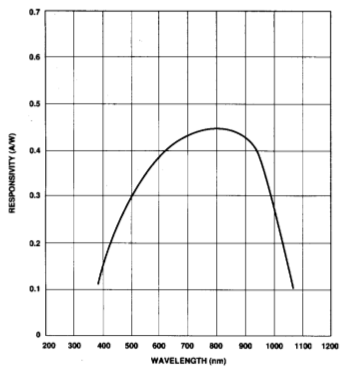
\includegraphics[scale=.45]{responsivity}
\caption{Responsività spettrale di OSD-15}
\label{fig:responsivity}
\end{figure}

Il rivelatore è stato collegato ad un circuito a transimpedenza come mostrato in figura \ref{fig:trans}

\begin{figure}[htp]
\centering
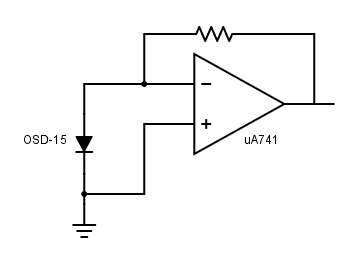
\includegraphics[scale=.45]{transimpedance}
\caption{Circuito a transimpedenza collegato al rivelatore}
\label{fig:trans}
\end{figure}

Come resistenza di feedback è stata scelta R = 55.6(4) $\Omega$.

Il laser impegato è un modello %nome modellooooo
con lunghezza d'onda di 779 nm, che cade quindi intorno al massimo di responsività spettrale del rivelatore. È stato collegato ad un circuito di controllo
%nome circuito
come mostrato in figura \ref{fig:laser}.

\begin{figure}[htp]
\centering
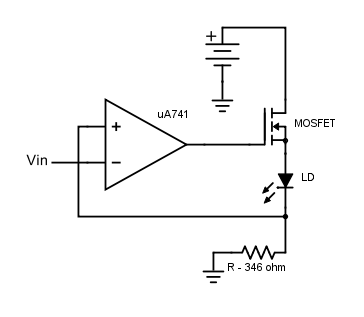
\includegraphics[scale=.5]{laser}
\caption{Circuito di controllo per il laser}
\label{fig:laser}
\end{figure} 

Date la corrente di soglia e la potenza emessa dal laser ad un altro valore di corrente maggiore di quello di soglia è facile determinare il valore della tensione $V_{in}$ perché il laser emetta la potenza desiderata. Infatti se $I_{thr}$ è la corrente di soglia, $I_f$ e $W_f$ un altro valore di corrente,con $I>I_{thr}$, e la relativa potenza, dal momento che la curva W-I per correnti superiori alla soglia è praticamente lineare, si può scrivere in questo regime:
\begin{equation}
W(I) = W_f \frac{I-I_{thr}}{I_f - I_{thr}}
\end{equation}

Dalle regole d'oro degli op-amp si ha che, facendo riferimento al circuito di figura \ref{fig:laser}:

\begin{equation}
I = \frac{V_{in}}{R}
\end{equation}

da cui è possibile ricavare sia la corrente che deve scorrere nel laser per ottenere una data potenza sia la tensione in ingresso per generare quella corrente. Ad esempio per ottenere 0.1 mW di potenza se $I_{thr} = 17\, mA$, $I_f = 25 \, mA$ e $W_f= 2.2 \, mW$ si ha:
\begin{gather}
I = 17.36 \, mA \\
V_{in} = 17.36 \, R
\end{gather}

dove R è in ohm e $V_{in}$ in mV. Nel nostro caso non avendo avuto a disposizione un valore affidabile per applicare le relazioni precedenti abbiamo dovuto determinare direttamente, tramite ,
%nome del coso usato da di lieto
la tensione in ingresso all'op-amp per ottenere una potenza emessa di 0.3 mW, risultando essere di 6.54 V. Il valore della resistenza di carico impiegata è R = (346 $\pm$ 3) $\Omega$.\\
Le misure in questa fase sono state effettuate tramite il VI \texttt{Vin$\_$Vout$\_$2C}, che permette di impostare sia la tensione in uscita ad un canale di output della scheda DAQ, nel nostro caso la CB22, che di rilevare le tensioni in due canali. Abbiamo quindi collegato la CB22 all'ingresso dell'opamp del circuito di controllo del laser e rilevato la tensione in uscita all'opamp collegato al rivelatore. Per le regole d'oro dell'op-amp, quest'ultima tensione è anche la d.d.p. ai capi della resistenza di feedback. È così possibile determinare direttamente la corrente generata dal rivelatore è tramite la responsività spettrale, che a 780 nm vale circa 0.45 A/W, la potenza incidente sul rivelatore.\\
Il laser e il rivelatore sono stati inseriti entro due fessure speculari di un supporto al cui interno è possibile incastrare le cuvette per le misure di assorbimento. La prima misura, effettuata a "vuoto", ha fornito $V_{out} = 3.70(5) V$ che per quanto detto in precedenza corrisponde ad una potenza incidente di 0.150(3) mW, la metà di quella che dovrebbe essere generata dal laser. Il motivo per cui si ottiene la metà di quello previsto potrebbe essere dovuto alla non perfetta collinearità del fascio laser e al fatto che non tutta la superficie del rivelatore è utile alla ricezione della radiazione.\\
La misura è stata ripetuta inserendo una cuvette vuota, effettuando le rilevazioni più volte inserendo più volte la cuvette, sia dal lato chiaro che opaco. I risultati sono riassunti in tabella \ref{tab:empty}.

\begin{table}[htp]
\centering
\caption{Misure con cuvette vuota}
\label{tab:empty}
\begin{tabular}{c|c}
\textbf{Lato chiaro} & 3.617(1) V ~ 0.1446(1) mW \\ 
\hline 
\textbf{Lato oscuro} & 3.408(1) V ~ 0.1362(1) mW \\ 
\end{tabular} 
\end{table}

Al ripetere delle misure il valore è rimasto stabile, le uniche variazioni rilevate nell'ultima cifra significativa dei risultati riportati sempre in tabella \ref{tab:empty}.

\subsection{Misure di assorbimento}

Per le misure di assorbimento si aveva a dispsizione delle cuvette con soluzioni di CuSO$_4$ in diverse concentrazioni. Le cuvette sono state inserite fra laser e rivelatore tramite l'apposito supporto ed è stata misurata la tensione all'uscita del'opamp nel circuito di figura \ref{fig:trans}, da cui come si è visto è possibile determinare la potenza incidente sul rivelatore. Nell'effettuare le misure le cuvette sono state posizionate più volte per verificare la ripetività della misura stessa. Abbiamo misurato l'assorbimento sia quando il laser incideva sui lati trasparenti che opachi delle cuvette. Riportiamo in tabella \ref{tab:001} i dati grezzi relativi al caso 0.01 M.

\begin{table}[htp]
\centering
\caption{Dati relativi al caso 0.01 M}
\label{tab:001}
\begin{tabular}{c|c}
\textbf{Lato Chiaro} &\textbf{ Lato Oscuro} \\ 
\hline 
3.494 & 3.228 \\ 
\hline 
3.514 & 3.293 \\ 
\hline 
3.511 & 3.247 \\ 
\hline 
3.501 & 3.271 \\ 
\hline 
3.491 & 3.193 \\ 
\hline 
3.501 & 3.232 \\ 
\hline 
3.478 & / \\		 
\hline 
3.472 & / \\	 
\hline 
3.457 & / \\ 
\end{tabular} 
\end{table}

Sono stati raccolti prima i primi 6 dati lato trasparente, poi quelli lato opaco e infine gli ultimi 3 lato trasparente. Si nota come la tensione registrata per questi ultimi dati sia significativamente diversa dai primi 6 dati, per di più lo stesso fenomeno è stato osservato anche per altre cuvette, cioè tensioni sensibilmente inferiori dopo aver fatto la misura con il lato opaco. È possibile che all'interno della stessa serie di misure (senza passare da un lato all'altro) involontariamente non si è spostato molto il punto in cui la radiazione laser incide sulla parete, mentre cambiando lato della cuvette si è ''persa memoria'' della posizione precedente rilevando così delle disomogeneità nella costituzione delle pareti. In ogni caso si è verificato che l'errore si mantenesse entro l' 1 $\%$.\\
Sono state infine effettuate le misure al variare della concentrazione, mediando sui diversi posizionamenti delle cuvette. In tabella \ref{tab:att} sono riportati i dati di $\frac{I}{I_0}$ in funzione della molarità, dove per $I_0$ sono stati presi i due valori di tabella \ref{tab:empty}, mentre un plot dei dati è mostrato in figura \ref{fig:att}.

\begin{table}[htp]
\centering
\caption{Attenuazioni in funzione della molarità}
\label{tab:att}
\begin{tabular}{c|c|c}
\textbf{Lato Chiaro} & \textbf{Lato oscuro} & \textbf{Molarità (mol)}\\ 	
\hline 
0.9635(2) & 0.9519(2) & 0.01 \\ 
\hline 
0.9323(2) & 0.9123(4) & 0.025 \\ 
\hline 
0.6588(2) & 0.5212(3) & 0.04 \\ 
\hline 
0.5040(2) & 0.3590(9) & 0.06 \\ 
\hline 
0.21778(5) & 0.1487(4) & 0.1 \\ 
\hline 
0.02806(2) & 0.02175(2) & 0.15 \\ 
\hline 
0.000838(1) & 0.000853(1) & 0.25 \\ 
\hline 
0.000777(1) & 0.000822(1) & 0.4 \\ 
\hline 
0.000710(1) & 0.000752(1) & 1 \\ 
\hline 
0.000709(1) & 0.000758(1) & 1.2 \\ 
\end{tabular} 
\end{table}

\begin{figure}[htp]
\centering
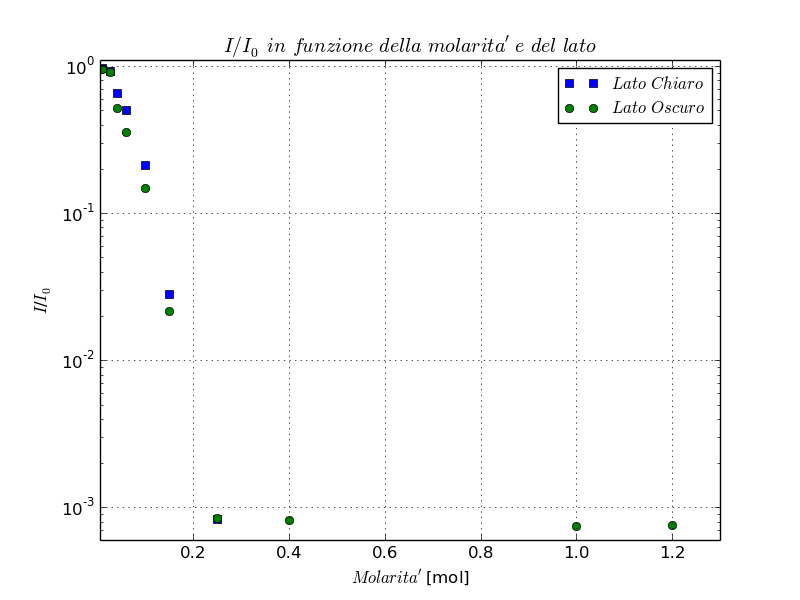
\includegraphics[scale=.6]{plotpowerrel}
\caption{Plot attenuazione in funzione della molarità}
\label{fig:att}
\end{figure}

Come si vede, per alte molarità l'attenuazione non segue un'andamento esponenziale, ma si mantiene approssimativamente costante. Questo potrebbe essere dovuto al fatto che a queste concentrazioni possono cadere alcune ipotesi su cui si basa la legge di Beer-Lambert, in particolare quella di centri assorbenti indipendenti. Per M = 0.01 si ha anche un significativo discostamento dall'andamento lineare dei dati centrali. Una possibile spiegazione in questo caso potrebbe essere che altre cause di attenuazione prevalgono rispetto a quelle dovute all'assorbimento da parte di CuSO$_4$, ad esempio la diffusione per scattering dei fotoni sulle molecole d'acqua o le pareti delle cuvette.\\
È stato fatto un fit dei dati relativi al lato chiaro lasciando libero il valore di $I_0$ secondo l'equazione:

\begin{equation}
\frac{I}{I_0}=C e^{- \alpha _u (\lambda) c x}
\end{equation}

tenendo conto dello spessore standard di 1 cm delle cuvette. Sono stati considerati solo i dati nella regione lineare, per cui sono stati esclusi il primo e gli ultimi tre dati. I risultati sono mostrati in figura \ref{fit:2} e in tabella \ref{tab:fit}.

\begin{figure}[!h]
\centering
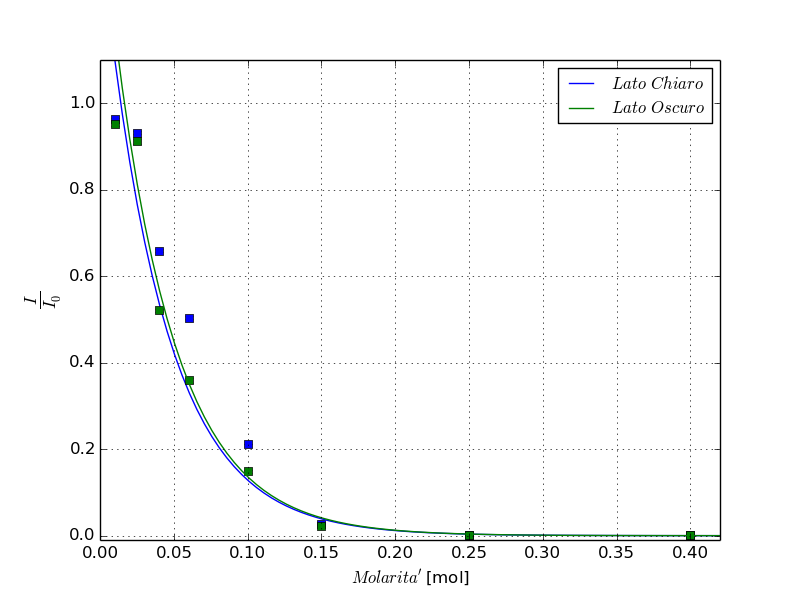
\includegraphics[scale=.6]{primofit}
\caption{Fit a due parametri dei dati sperimentali}
\label{fit:2}
\end{figure}

\begin{table}[!h]
\centering
\caption{Risultati fit, $\lambda$ = 779 nm}
\label{tab:fit}
\begin{tabular}{c|c|c}
\textbf{Lato} & \textbf{Chiaro} & \textbf{Oscuro} \\
\hline
$\alpha _u (\lambda)$ [cm$^{-1}$ mol$^{-1}$]& 24(2) & 24(2) \\ 
\hline 
C & 1.5(5) & 1.5(5) \\ 
\end{tabular} 
\end{table}

È interessante notare come i valori del coefficiente di assorbimento nei due casi sia venuto del tutto identico, cosa che effettivamente ci aspettava dal momento che normalizzando con l'assorbimento delle cuvette vuote si dovrebbe essere eliminata una differenza fra i due lati. Il coefficiente \emph{C} viene compatibile con 1, quindi sembrerebbe che il contributo dell'acqua all'attenuazione della radiazione incidente sia trascurabile.

\section{Rivelazione di piccoli segnali - 2}
\subsection{Misure del prodotto}

\begin{figure}[htp]
\centering
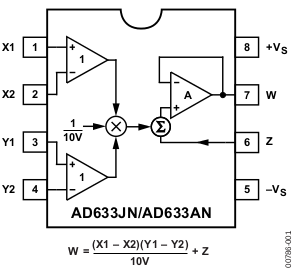
\includegraphics[scale=.6]{pinconf}
\caption{Configurazione dei pin di AD633}
\label{fig:pin}
\end{figure}

Si faccia riferimento alla figura \ref{fig:pin} per la configurazione dei pin nel AD633. Si vuole adesso configurare il circuito in modo tale da impiegare anche il canale B del generatore ATTEN. La configurazione immediata è naturalmente quella di mettere i pin 2 e 4 a terra, il pin 1 ad esempio al canale B dell'ATTEN e al pin 3 il canale A sempre del generatore. Se i segnali generati sono segnali sinusoidali della stessa frequenza ma sfasati fra loro, è facile vedere come il segnale in uscita dal dispositivo avrà un offset che dipende dalla fase relativa dei due segnali. Infatti se

\begin{gather}
V_A = A \sin (\omega t + \varphi) \\
V_B = B \sin (\omega t)
\end{gather}

sono i segnali inviati al dispositivo, il segnale in uscita è dato dalla formula che appare in figura \ref{fig:pin}, in questo caso:

\begin{equation}
\begin{split}
V_{out} & = C \sin (\omega t + \varphi) \sin (\omega t) \\
		& = \frac{C}{2} ( \cos \varphi - \cos (2 \omega t + \varphi))
\end{split}
\end{equation}

dove C = AB. Quindi la presenza di una fase relativa implica la comparsa di un offset, che è massimo quando la fase è nulla. È opportuno quindi avere un modo per avere sotto controllo la fase relativa dei segnali in ingresso al AD633. Fortunatamente il generatore ATTEN consente di regolare direttamente la fase dei segnali trasmessi tramite i due canali per mezzo di una opportuna combinazione di pulsanti. Un'alternativa è collegare ad uno dei segnali in ingresso un filtro (derivatore o integratore) che oltre ad un'attenuazione introduce una fase senza cambiare, nel caso di segnali puramente monocromatici, la forma dell'onda. In questo caso la fase si può regolare mettendo come resistenza un potenziometro.\\
È interessante considerare anche il caso in cui i due segnali non hanno esattamente la stessa frequenza, dal momento che questo è proprio il caso che si presenta impostando frequenze uguali per i due canali dell'ATTEN in quanto non ci si può naturalmente aspettare che questo sia effettivamente rispettato. Sempre per mezzo della formula di cui in figura \ref{fig:pin}, se i due segnali sono:

\begin{gather}
V_A = A \sin (\omega _1 t + \varphi) \\
V_B = B \sin (\omega _2 t)
\end{gather}

si ottiene:

\begin{equation}
\begin{split}
V_{out} & = C \sin (\omega _1 t + \varphi) \sin (\omega  _2 t ) \\
		& = \frac{C}{2} ( \cos ((\omega _1 - \omega _2 ) t + \varphi) - \cos ((\omega _1 + \omega _2) t + \varphi))
\end{split}
\end{equation}

Ovvero la somma di un segnale di frequenza $\omega _1 + \omega _2 \approx 2 \omega$ con un segnale di frequenza molto più piccola. Ciò che ci si aspetta di vedere è quindi un segnale di frequenza $2 \omega$ con un offset che varia periodicamente e lentamente. Questo è effettivamente quanto si è osservato (è disponibile su gentile concessione degli autori un video che lo dimostra).\\ Nelle figure  \ref{subfig2} i grafici restituiti dal VI \texttt{Acquis$\_$base4} al variare della fase dei due segnali in ingresso.

\begin{figure}[!h]
    \centering
    
    ~ %add desired spacing between images, e. g. ~, \quad, \qquad, \hfill etc. 
      %(or a blank line to force the subfigure onto a new line)
    \begin{subfigure}[b]{0.45\textwidth}
        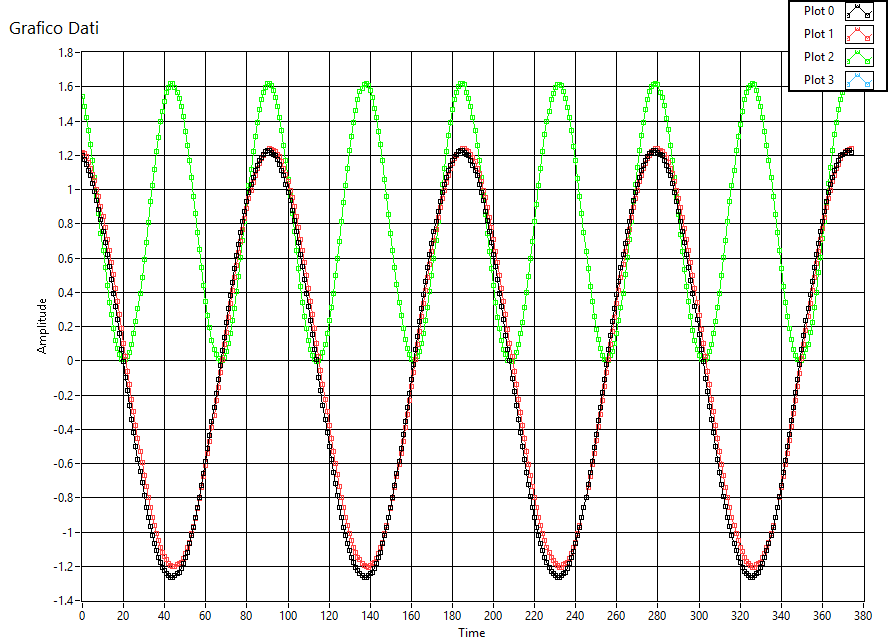
\includegraphics[width=\textwidth]{es24_circa0grad}
        \caption{$\Delta \varphi \approx 0^{\circ}$}
        \label{fig:tiger}
    \end{subfigure}\quad
    ~ %add desired spacing between images, e. g. ~, \quad, \qquad, \hfill etc. 
    %(or a blank line to force the subfigure onto a new line)
    \begin{subfigure}[b]{0.45\textwidth}
        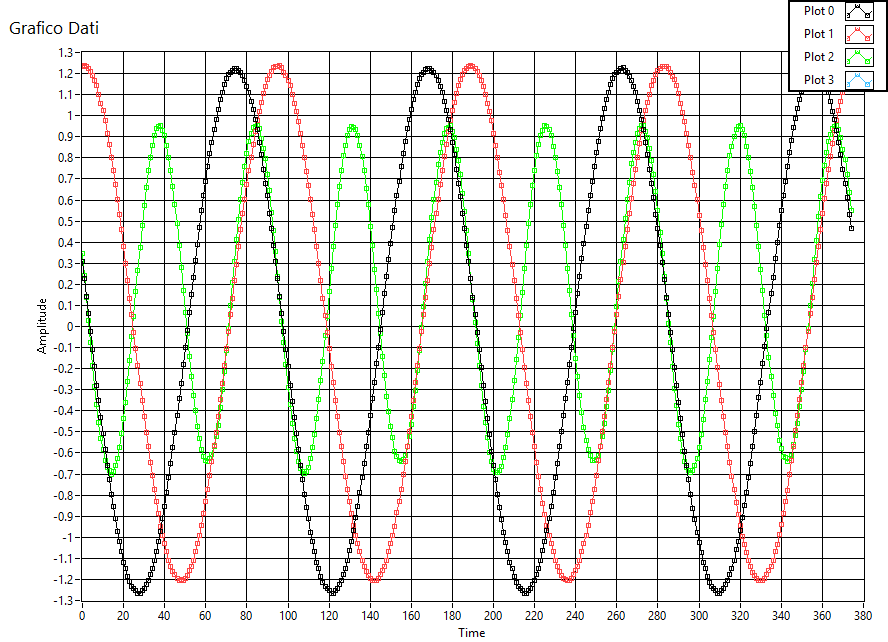
\includegraphics[width=\textwidth]{es24_circa80grad}
        \caption{$\Delta \varphi \approx 80^{\circ}$}
        \label{fig:mouse}
    \end{subfigure}
    \begin{subfigure}[b]{0.45\textwidth}
        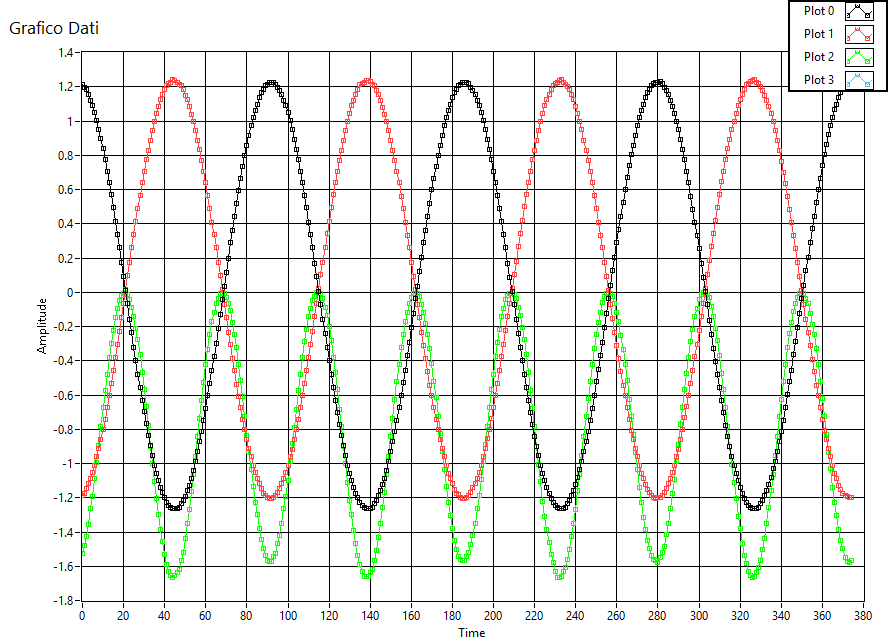
\includegraphics[width=\textwidth]{es24_circa180grad}
        \caption{$\Delta \varphi \approx 180^{\circ}$}
        \label{fig:mouse}
    \end{subfigure}
    \quad
   \begin{subfigure}[b]{0.45\textwidth}
        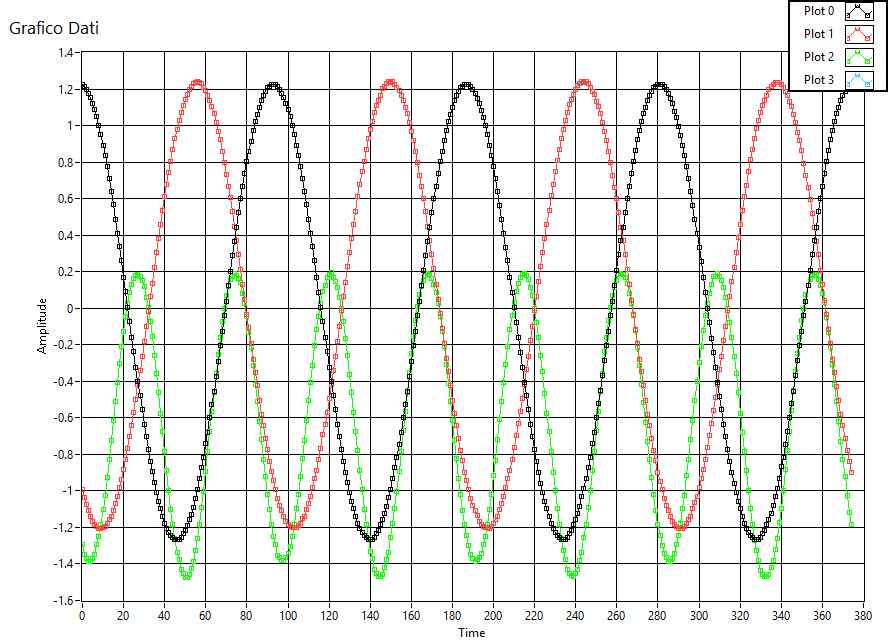
\includegraphics[width=\textwidth]{es24_circa220grad}
        \caption{$\Delta \varphi \approx 220^{\circ}$}
        \label{fig:gull}
    \end{subfigure}
    \caption{Uscita AD633 in funzione della fase relativa. In rosso e nero gli ingressi, in verde l'uscita}
    \label{subfig2}
\end{figure}
Per misurare l'offset dovuto alla differenza di fase dei segnali in ingresso al AD633 è possibile servirsi del circuito in figura \ref{es26}.

\begin{figure}[!h]
\centering
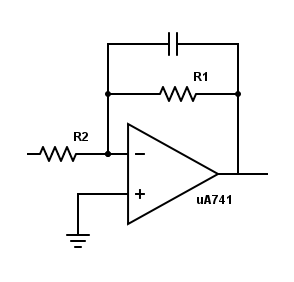
\includegraphics[scale=.6]{es25}
\caption{Schema del circuito "mediatore"}
\label{es26}
\end{figure}

Si ha che esso esegue una media del segnale in ingresso fatta su un tempo $\tau  = R_2C$, dopodichè il segnale mediato risulta moltiplicato per un fattore $-\frac{R_1}{R_2}$. Abbiamo scelto come valori delle impedenze C = 100nF, $R_1$ = 224 k$\Omega$, $R_2$ = 55.6 $\Omega$. Pertanto $\tau$=5.56 ms, circa 4 volte il periodo del segnale, $\tau_s$ = 1.25 ms, e un fattore di amplificazione di -4. In figura \ref{subfig3} sono mostrati i grafici restituiti da \texttt{Acquis$\_$base4}, si vede come effettivamente i risultati sono in accordo con quanto previsto.

\begin{figure}[!h]
    \centering
    
    ~ %add desired spacing between images, e. g. ~, \quad, \qquad, \hfill etc. 
      %(or a blank line to force the subfigure onto a new line)
    \begin{subfigure}[b]{0.7\textwidth}
        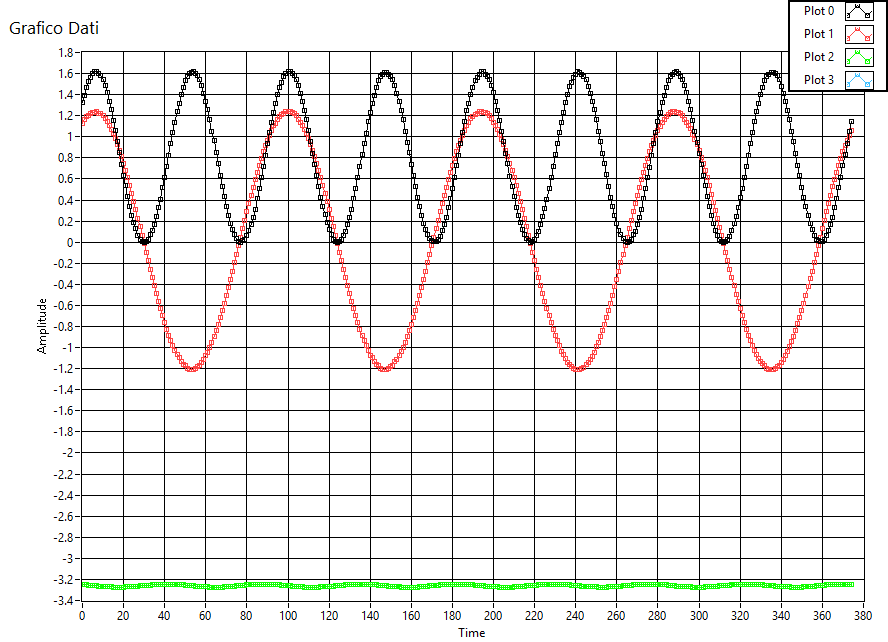
\includegraphics[width=\textwidth]{es25_800hz_100nF_0deg}
        \caption{$\Delta \varphi \approx 0^{\circ}$}
        \label{fig:tiger}
    \end{subfigure}\quad
    ~ %add desired spacing between images, e. g. ~, \quad, \qquad, \hfill etc. 
    %(or a blank line to force the subfigure onto a new line)
    \begin{subfigure}[b]{0.7\textwidth}
        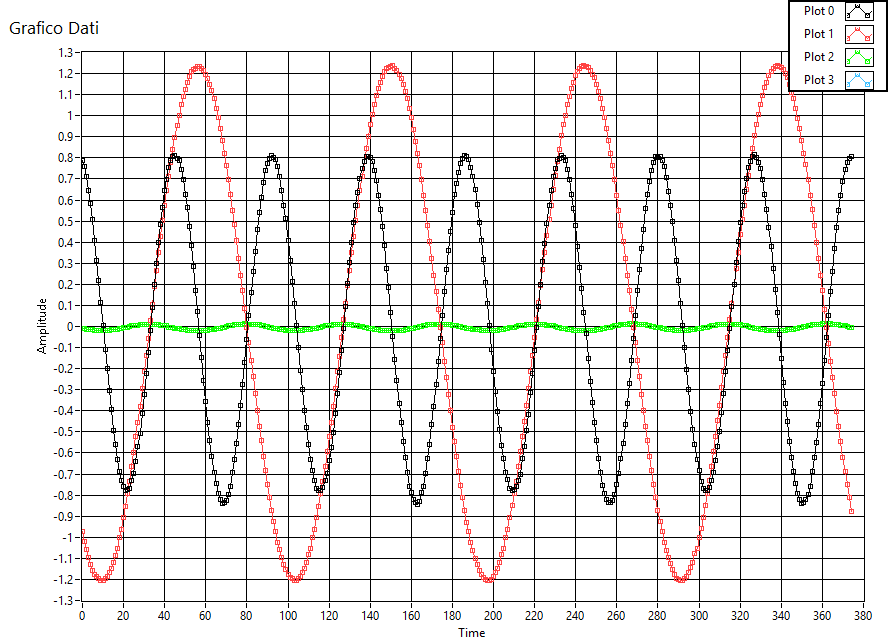
\includegraphics[width=\textwidth]{es25_800hz_100nF_90deg}
        \caption{$\Delta \varphi \approx 90^{\circ}$}
        \label{fig:mouse}
    \end{subfigure}
    \begin{subfigure}[b]{0.7\textwidth}
        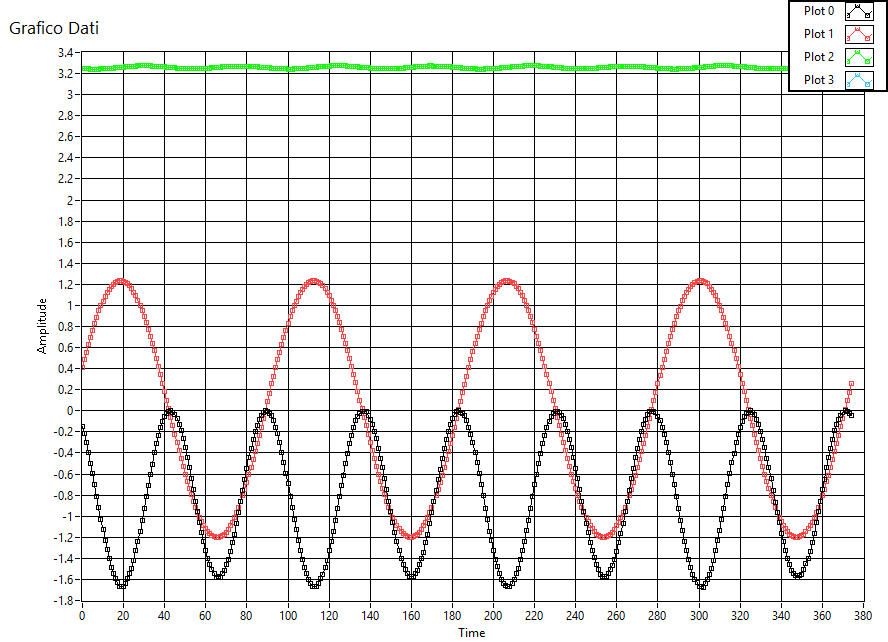
\includegraphics[width=\textwidth]{es25_800hz_100nF_180deg}
        \caption{$\Delta \varphi \approx 180^{\circ}$}
        \label{fig:mouse}
    \end{subfigure}
\caption{Uscita AD633 in funzione della fase relativa. In rosso uno dei due segnali in ingresso, in nero l'uscita dal AD633, in verde l'uscita dal mediatore}
\label{subfig3}
\end{figure}


\end{document}